\documentclass[oneside]{article}
\usepackage{wallpaper}
\usepackage{geometry}
\usepackage[
    unicode=true,
    bookmarks=true,
    bookmarksnumbered=false,
    bookmarksopen=true,
    bookmarksopenlevel=1,
    breaklinks=false,
    pdfborder={0 0 0},
    backref=false,
    colorlinks=false
    ]{hyperref}
\usepackage{lastpage}
\usepackage{hyphenat}
\usepackage{hyphsubst}
\usepackage{tabularx}
\usepackage{moresize}
\usepackage[document]{ragged2e}
\usepackage[scaled]{helvet}
\usepackage{fontawesome5}
% \usepackage{lmodern}
\usepackage[defaultfam,tabular,oldstyle]{montserrat}
\usepackage[T1]{fontenc}
\renewcommand*\oldstylenums[1]{{\fontfamily{Montserrat-TOsF}\selectfont #1}}
\usepackage{titlesec}
\usepackage{xcolor}
\usepackage{tikz}
\setlength{\parindent}{0pt}
\titleformat{\section}{\normalfont}{}{0pt}{}
\renewcommand{\arraystretch}{1.4}
\setlength\fboxrule{0pt}
\setlength\fboxsep{12pt}
\titlespacing{\section}{0pt}{1.5ex plus .1ex minus .2ex}{1pc}
\newcolumntype{Y}{>{\RaggedRight\arraybackslash}X}
% Change PDF Meta Info here
\hypersetup{
    pdftitle={Muhammad Huzaifa - CV - English},
    pdfauthor={Muhammad Huzaifa},
    pdfsubject={CV}
}
% Paper size
\geometry{
    a4paper,
    left=0pt,
    right=0pt,
    top=0pt,
    bottom=0pt,
    nohead,
    nomarginpar
}
% Background Color of the Sidebar Column
\definecolor{sidebg}{cmyk}{1, 0.02, 0, 0.56}
% Background Color of the Main Column
\definecolor{mainbg}{cmyk}{0, 0, 0.07, 0.04}
% Text Color of the Main Column
\definecolor{maintext}{cmyk}{1, 0.02, 0, 0.8}
% Text Color of the Sidebar Column
\definecolor{sidetext}{cmyk}{0, 0, 0.07, 0.04}
\pagecolor{mainbg}
\begin{document}
\setlength{\topskip}{0pt}\setlength{\footskip}{0pt}%
\fcolorbox{red}{sidebg}{%
    \begin{minipage}[t][\textheight-2\fboxsep-2\fboxrule][t]{\dimexpr0.40\textwidth-2\fboxrule-2\fboxsep\relax}
        \color{sidetext}
        % NAME
        {\bfseries\scshape\HUGE Muhammad} \\
        {\bfseries\scshape\Huge Huzaifa} \qquad {he/him}
        \vspace{2pt} \\
        \begin{center}
            \begin{tikzpicture}
                \clip (0,0) circle (3cm) node[anchor=center] {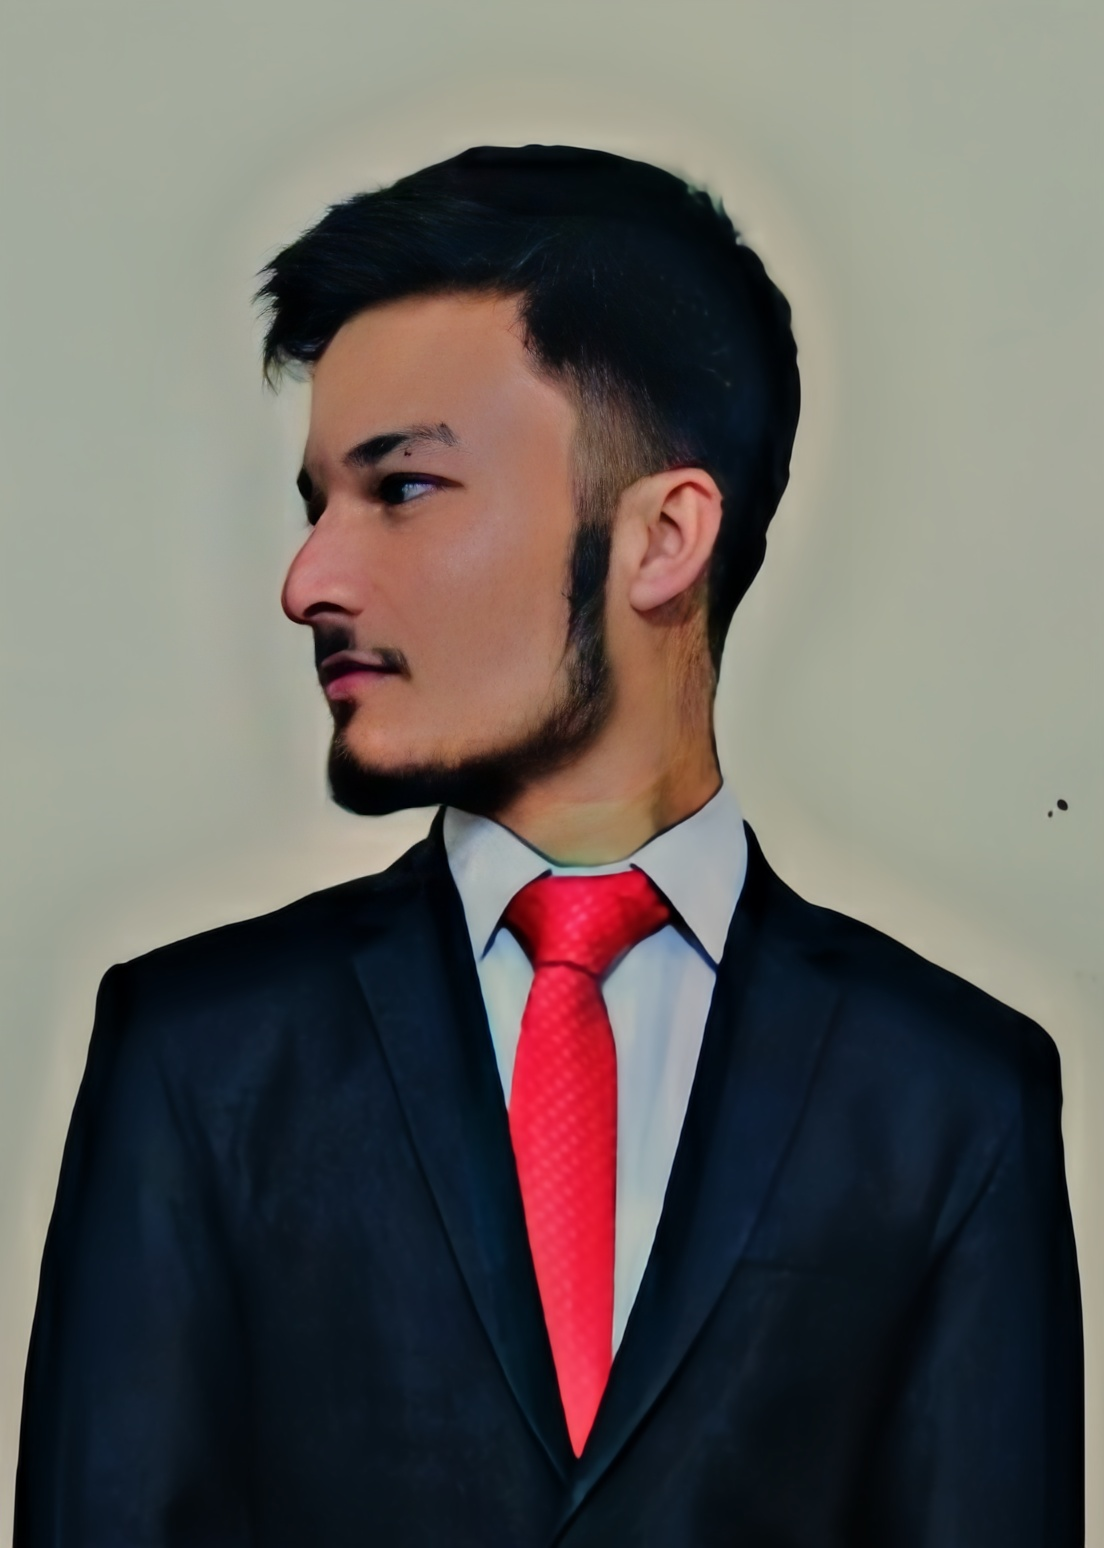
\includegraphics[width=6cm]{pf.jpg}};
            \end{tikzpicture}
        \end{center}
        \vspace{2pt}
        % PERSONAL INFROMATION
        \phantomsection{}
        \addcontentsline{toc}{section}{Personal info}
        \section*{\large Personal info}
        \begin{tabularx}{\textwidth}{cY}
            \faStarOfLife{} & 03/02/2002                                            \\
            \faPhone{}      & 03007005268                                           \\
            \faEnvelope{}   & \href{sadaat185336@gmail.com}{sadaat185336@gmail.com} \\
            \faMapMarker{}  & Peshawar |Mera Utmanzai Dist Charsadda                \\
        \end{tabularx}
        \vspace{.3cm} \\
        \rule{\linewidth}{0.4pt} \\
        %  LINKS
        \phantomsection{}
        \addcontentsline{toc}{section}{Links}
        \section*{\large Links}
        \begin{tabular}{cl}
            \faGithub{}   & \href{https://github.com/rogueinnovator}{rogue-innovator}                                \\
            \faLinkedin{} & \href{https://www.linkedin.com/in/muhammad-huzaifa-ali-49aa94259/}{Muhammad Huzaifa Ali} \\
            \faTwitter{}  & \href{https://www.twitter.com/in/rogue-innovator}{rogueinnovator}                        \\
            \faSlack{}    & \href{https://app.slack.com/client/T06MHHWUB7E/C06M8HF9REJ}{Muhammad Huzaifa}
        \end{tabular}
        \vspace{10pt} \\
        \rule{\linewidth}{0.4pt} \\
        %SKILLS
        \phantomsection{}
        \addcontentsline{toc}{section}{Skills}
        \section*{\large Skills}
        \begin{tabularx}{\textwidth}{cY}
            \faCode{}       & JavaScript, Solidity, Java, SQL     \\
            \faPen*{}       & \LaTeX, Tailwindcss, BootStrap, CSS \\
            \faFont{}       & \ LibreOffice, Gedit                \\
            \faCogs{}       & Linux \hspace{4pt}  \faLinux{}      \\
            \faLaptopCode{} & Visual Studio Code                  \\
            \faToolbox{}    & DrawIO, Ganache, Docker
        \end{tabularx}
        \vspace{1pt} \\
        \rule{\linewidth}{0.4pt}
        \phantomsection{}
        \addcontentsline{toc}{section}{Skills}
        \section*{\large Hobbies}
        \begin{tabularx}{\textwidth}{cY}
            \faUsers{} & Sketching, Cricket, Photography, Writing, Love mini electrical and Arduino projects \\
        \end{tabularx}
        \vfill
        {\tiny Made in \LaTeX by rogue-innovator}

    \end{minipage}
}
\hfill
\fcolorbox{red}{mainbg}

\begin{minipage}[t][\dimexpr\textheight-2\fboxrule-2\fboxsep\relax][t]{\dimexpr0.6\textwidth-2\fboxrule-2\fboxsep\relax}
    \color{maintext}
    % WORK EXPERIENCE
    \phantomsection{}
    \addcontentsline{toc}{section}{Experience}
    \section*{\scshape\Large Experience \rule{\linewidth}{0.4pt}}
     %
     {\large \textbf{React Experience}} \\
    \vspace{7pt}
    \begin{itemize}
        \setlength{\itemsep}{-1pt}
        \item  Components and Props
        \item State and Lifecycle
        \item Handlinents
        \item React Hooks
        \item React Routing
        \item API Requests
        \item State Management using Redux
    \end{itemize}
    %
    {\large \textbf{Node Experience}} \\
    \begin{itemize}
        \setlength{\itemsep}{-1pt}
        \item Express.js
        \item RESTful APIs
        \item Working with MongoDB
        \item CRUD operations
        \item Authentication Authorization
        \item Error handling
        \item File Uploads
        \item Validation (using express-validator)
    \end{itemize}
    %
    {\large \textbf{BlockChain}} \\
    \begin{itemize}
        \setlength{\itemsep}{-1pt}
        \item Basic concepts
        \item Solidity Basics
              \begin{enumerate}
                  \item Syntax, DataTypes, Variables
                  \item Writing Deploying Simple Smart Contract
              \end{enumerate}
        \item Ethereum BlockChain
        \item Web3.js
        \item Truffle FrameWork
        \item Ganache
        \item Concepts of Chainlink and Oracles
    \end{itemize}


    % EDUCATION
    \phantomsection{}
    \addcontentsline{toc}{section}{Education}
    \section*{\scshape\Large Education \rule{\linewidth}{0.4pt}}
     {\large \textbf{Al karim public High school Charsadda }} \\
    \vspace{4pt}
    {\scshape\fontseries{light} \qquad  2006 \textemdash{}  2018}\\
    \vspace{4pt}
    {Matric\\}
    \vspace{4pt}
    {Grades:\hspace{3pt} 1001 out of 1100} \\[1ex]
    {\large \textbf{Ismalia College Peshawar}} \\
    \vspace{4pt}
    { \qquad  2018 \textendash{}  2020} \\
    \vspace{4pt}
    {Pre\textemdash{}Engneering\\}
    \vspace{4pt}
    {Grades:\hspace{3pt} 883 out of 1100} \\[1ex]
    {\large \textbf{University of Peshawar}} \\
    \vspace{4pt}
    { \qquad  2020 \textendash{}  2024} \\
    \vspace{4pt}
    {BS Computer Science\\}
    \vspace{4pt}
    {GPA:\hspace{3pt} 3.5} \\[1ex]
\end{minipage}

\end{document}
